%
\chapter{Projeto B}

Neste projeto, iremos construir uma rede com dois nós sensores para monitorar a temperatura, umidade e luminosidade de um ambiente.  Vamos construir um nó sensor para coletar informações de temperatura e umidade e outro nó para coletar informações de luminosidade do ambiente, os dois nós devem se comunicar com o controlador. O intuito desse projeto é apresentar como incluir mais nós em uma rede e como atualizar as informações do controlador para suportar os novos nós. 

\section{Materiais}

Para esse projeto vamos utilizar os seguintes materiais:
\begin{itemize}
\item 3 Arduinos;
\item Sensor de temperatura e umidade DTH11;
\item Sensor de luminosidade LDR;
\item 3 Rádios RF;
\item Jumpers.
\end{itemize}

Para obter mais informações sobre os materiais consulte o capítulo ~\ref{MateSof}.

\section{Implementação}

\subsection{Gateway}
\vbox{
\indent \rule{10.4cm}{0.6pt}\par
\textbf{Esquemático}\par%\vspace{-0.66\baselineskip}
\rule[0.90\baselineskip]{10.4cm}{0.6pt}
}

\begin{figure}[ht]
      \centering
      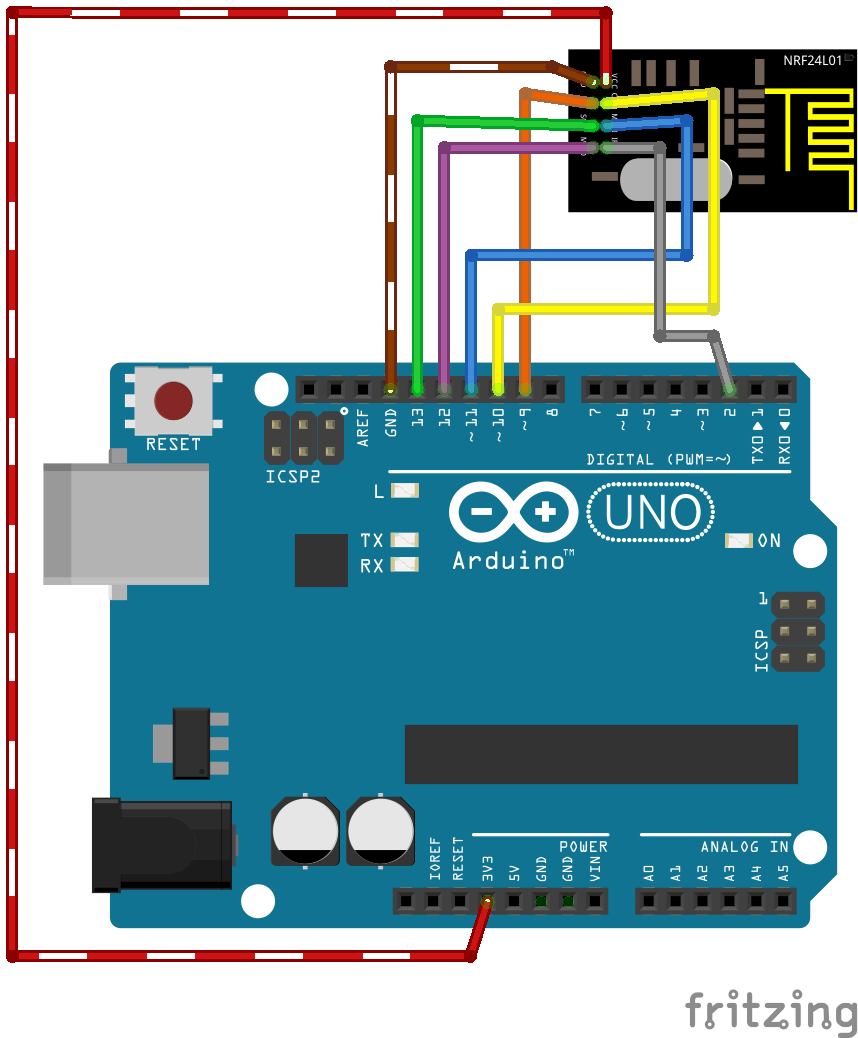
\includegraphics[scale=0.70]{figuras/gateway.png}
      \caption{Gateway}
      \label{fig:gateway2}
\end{figure}
\pagebreak
\vbox{
\indent \rule{10.4cm}{0.6pt}\par
\textbf{Código}\par%\vspace{-0.66\baselineskip}
\rule[0.90\baselineskip]{10.4cm}{0.6pt}
}

\lstinputlisting[language=C++, caption={Gateway}]{code/teste.ino}

\subsection{Nó com sensor DTH11}

\vbox{
\indent \rule{10.4cm}{0.6pt}\par
\textbf{Esquemático}\par%\vspace{-0.66\baselineskip}
\rule[0.90\baselineskip]{10.4cm}{0.6pt}
}

\begin{figure}[ht]
      \centering
      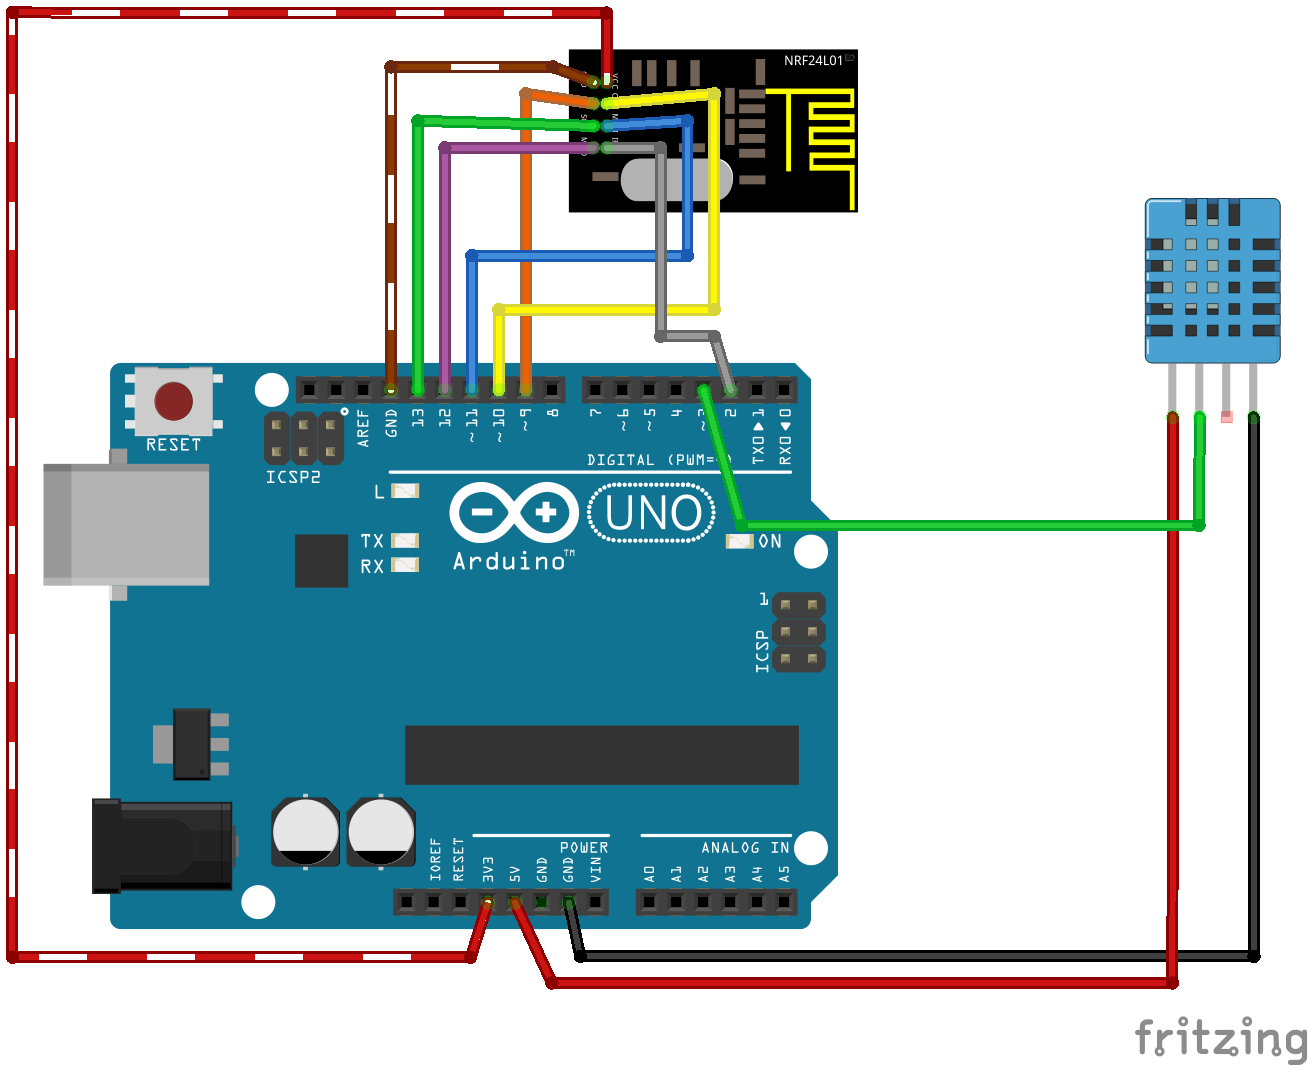
\includegraphics[scale=0.70]{figuras/DTH11_bb.png}
      \caption{Sensor DTH11}
      \label{fig:dth112}
\end{figure}
\pagebreak

\vbox{
\indent \rule{10.4cm}{0.6pt}\par
\textbf{Código}\par%\vspace{-0.66\baselineskip}
\rule[0.90\baselineskip]{10.4cm}{0.6pt}

}

\lstinputlisting[language=C++, caption={DTH11}]{code/dth11.ino}


\subsection{Nó com sensor LDR}

\vbox{
\indent \rule{10.4cm}{0.6pt}\par
\textbf{Esquemático}\par%\vspace{-0.66\baselineskip}
\rule[0.90\baselineskip]{10.4cm}{0.6pt}
}

\begin{figure}[ht]
      \centering
      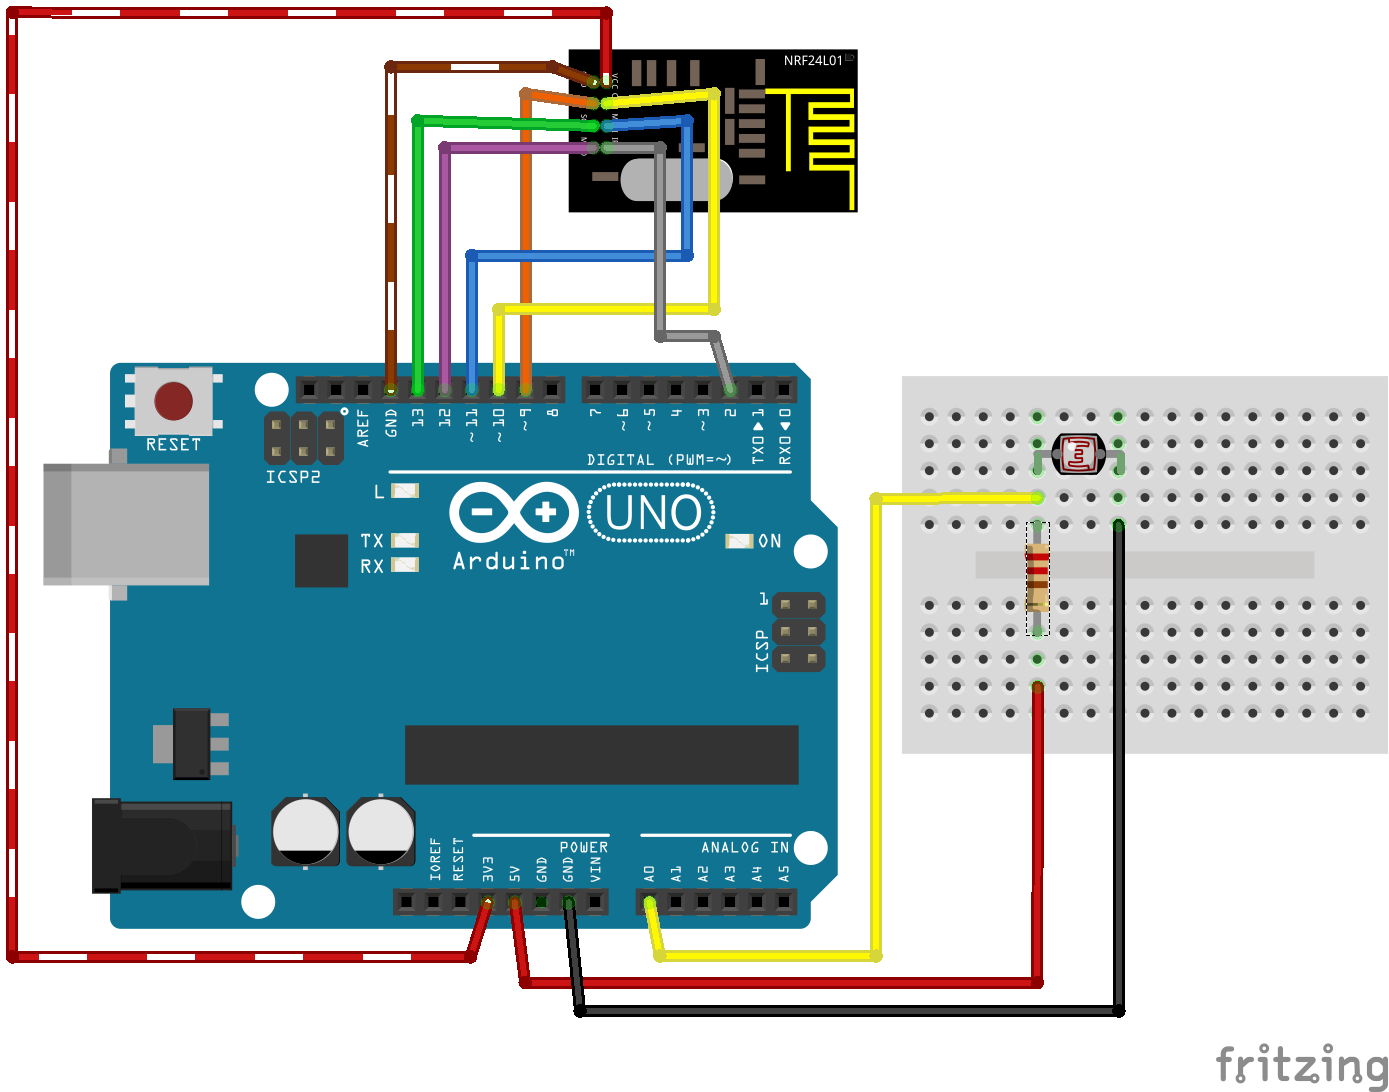
\includegraphics[scale=0.70]{figuras/ldr.png}
      \caption{Sensor LDR}
      \label{fig:ldr2}
\end{figure}
\pagebreak

\vbox{
\indent \rule{10.4cm}{0.6pt}\par
\textbf{Código}\par%\vspace{-0.66\baselineskip}
\rule[0.90\baselineskip]{10.4cm}{0.6pt}

}

\lstinputlisting[language=C++, caption={LDR}]{code/ldr.ino}


\subsection{Controlador}

Arquivo de configuração do Pimatic

\lstinputlisting[language=C++, caption={json.conf}]{code/jsonB.json}